\section*{Appendix A - Listings}

\begin{lstlisting}[language=C, caption={Almost Equal algorithm}, label={lst:almost_equal}]
bool almost_equal(float x, float y) {
    int maxUlps = 2048;
    int xBits = *(int *)&x;  // Evil bit level hacking from Quake III Q_sqrt
    int yBits = *(int *)&y;  // Evil bit level hacking from Quake III Q_sqrt
    int minValue = 1 << 31;
    if (xBits < 0) xBits = minValue - xBits;
    if (yBits < 0) yBits = minValue - yBits;

    int difference = xBits - yBits;
    return difference != minValue && fabsf(difference) <= maxUlps;
}
\end{lstlisting}

\begin{lstlisting}[language=C, caption={Code to measure allocating and freeing memory}, label={lst:cudaMalloc}]
void malloc_scaling_with_dimension(matrix_t *matrix) {
    device_matrix_t device_matrix =
        cuda_matrix_init(matrix->rows, matrix->columns);
    cuda_matrix_free(device_matrix);
}
\end{lstlisting}

\begin{lstlisting}[language=C, caption={Code to measure moving memory}, label={lst:cudaMemcopy}]
void memcpy_scaling_with_dimension(matrix_t *matrix) {
    device_matrix_t device_matrix =
        cuda_matrix_init(matrix->rows, matrix->columns);
    cuda_matrix_host_to_device(device_matrix, matrix);
    cuda_matrix_device_to_host(matrix, device_matrix);
    cuda_matrix_free(device_matrix);
}
\end{lstlisting}

\begin{lstlisting}[language=C, caption={Code to measure spawning more blocks}, label={lst:noop}]
__global__ void noop_kernel() {}

void launch_kernel_scaling_with_dimension(int dimension) {
    noop_kernel<<<dimension, 1024>>>();
}
\end{lstlisting}

\begin{lstlisting}[language=C, caption={Code to measure the launch of asynchronous kernels}, label={lst:asynchronous kernels}]
void launch_x_kernels(int dimension) {
    for (int i = 0; i < dimension; i++)
    {
        noop_kernel<<<1, 1>>>();
    }
}
\end{lstlisting}

\begin{lstlisting}[language=C, caption={Code to measure the launch of synchronous kernels}, label={lst:synchronous kernels}]
void launch_x_kernels_sequentially(int dimension) {
    for (int i = 0; i < dimension; i++)
    {
        noop_kernel<<<1, 1>>>();
        cudaDeviceSynchronize();
    }
}
\end{lstlisting}

\begin{lstlisting}[language=C, caption={CPU addition algorithm}, label={lst:cpu_addition}]
bool matrix_addition(matrix_t *matrix_a, matrix_t *matrix_b, matrix_t *matrix_c) {
    if (matrix_a == NULL) return false;
    if (matrix_b == NULL) return false;
    if (matrix_c == NULL) return false;
    if (!matrix_equal_dimensions(matrix_a, matrix_b)) return false;
    if (!matrix_equal_dimensions(matrix_a, matrix_c)) return false;

    int rows = matrix_a->rows;
    int columns = matrix_a->columns;

    for (int i = 0; i < rows * columns; i++)
        matrix_c->values[i] = matrix_a->values[i] + matrix_b->values[i];

    return true;
}
\end{lstlisting}

\begin{lstlisting}[language=C, caption={Algorithm runner for GPU algorithms.}, label={lst:algorithm_runner}]
bool cuda_matrix_algorithm_runner(
    matrix_t* matrix_a, 
    matrix_t* matrix_b,
    matrix_t* matrix_c, 
    int kernel_param1, 
    int kernel_param2, 
    int kernel_param3,
    void (*kernel)(device_matrix_t, device_matrix_t, device_matrix_t, int, int, int),
    dim3 grid_size, dim3 block_size) {
    
    // null checks
    if (matrix_a == NULL || matrix_b == NULL || matrix_c == NULL) return false;

    // init matrices on device
    device_matrix_t device_matrix_a =
        cuda_matrix_init(matrix_a->rows, matrix_a->columns);
    device_matrix_t device_matrix_b =
        cuda_matrix_init(matrix_b->rows, matrix_b->columns);
    device_matrix_t device_matrix_c =
        cuda_matrix_init(matrix_c->rows, matrix_c->columns);

    // null check matrix initialization
    if (device_matrix_a == NULL || device_matrix_b == NULL ||
        device_matrix_c == NULL)
        return false;

    // copy matrix from host to device
    cuda_matrix_host_to_device(device_matrix_a, matrix_a);
    cuda_matrix_host_to_device(device_matrix_b, matrix_b);

    // launch kernel
    kernel<<<grid_size, block_size>>>(device_matrix_a, device_matrix_b,
        device_matrix_c, kernel_param1, kernel_param2, kernel_param3);

    // cuda result matrix from device to host
    cuda_matrix_device_to_host(matrix_c, device_matrix_c);

    // free matrices from device
    cuda_matrix_free(device_matrix_a);
    cuda_matrix_free(device_matrix_b);
    cuda_matrix_free(device_matrix_c);

    return true;
}
\end{lstlisting}

\begin{lstlisting}[language=C, caption={QR Decomposition on the CPU}, label={lst:qr_decomposition_cpu}]
// returns true if the matrix is singular
bool matrix_qr_decomposition(matrix_t *matrix, float *diagonal, float *c) {
    float column_length;  // sigma in book
    float column_length_squared, element;
    int n = matrix->columns;
    float scale;
    bool is_singular = false;
    // for every column
    for (int k = 0; k < n; k++) {
        scale = 0.0f;
        // scale is the max absolute value of the column
        for (int i = k; i < n; i++)
            scale = fmaxf(scale, fabsf(matrix->values[INDEX(i, k, n)]));

        if (scale == 0.0) {
            is_singular = true;
            c[k] = diagonal[k] = 0.0f;
            continue;
        }
        // Normalize column
        for (int i = k; i < n; i++) matrix->values[INDEX(i, k, n)] /= scale;

        // column length below diagonal
        column_length_squared = 0.0f;  // sum in book.
        for (int i = k; i < n; i++) {
            element = matrix->values[INDEX(i, k, n)];
            column_length_squared += element * element;
        }

        // column length below diagonal, with the sign of diagonal k
        column_length =
            SIGN(sqrtf(column_length_squared), matrix->values[INDEX(k, k, n)]);

        // add column length to diagonal k
        matrix->values[INDEX(k, k, n)] += column_length;

        c[k] = matrix->values[INDEX(k, k, n)] * column_length;

        diagonal[k] = -scale * column_length;

        // Calculate Q[k] = I - (u[k] (x) u[k]) / c[k]
        for (int j = k + 1; j < n; j++) {
            // inner product for column j below diagonal
            float inner_product = 0.0f;
            for (int i = k; i < n; i++) {
                inner_product += matrix->values[(INDEX(i, k, n))] *
                                 matrix->values[(INDEX(i, j, n))];
            }

            // division
            float tau = inner_product / c[k];

            for (int i = k; i < n; i++) {
                matrix->values[(INDEX(i, j, n))] -=
                    tau * matrix->values[(INDEX(i, k, n))];
            }
        }
    }

    if (!is_singular) is_singular = diagonal[n - 1] == 0.0f;
    return is_singular;
}
\end{lstlisting}

\begin{lstlisting}[language=C, caption={QR Decomposition GPU Single Core implementation}, label={lst:qr_gpu_singlecore}]
__global__ void cuda_matrix_qr_decomposition_single_core_kernel(
    device_matrix_t matrix, float *diagonal, float *c, int dimension,
    bool *is_singular) {
    float column_length;  // sigma in book
    float column_length_squared, element;
    int n = dimension;
    float scale;
    *is_singular = false;

    // for every column
    for (int k = 0; k < n; k++) {
        scale = 0.0f;
        // scale is the max absolute value of the column
        for (int i = k; i < n; i++) {
            scale = fmaxf(scale, fabsf(matrix[INDEX(i, k, n)]));
        }
        if (scale == 0.0) {
            *is_singular = true;
            c[k] = diagonal[k] = 0.0f;
            continue;
        }
        // Normalize column
        for (int i = k; i < n; i++) matrix[INDEX(i, k, n)] /= scale;

        // column length below diagonal
        column_length_squared = 0.0f;  // sum in book.
        for (int i = k; i < n; i++) {
            element = matrix[INDEX(i, k, n)];
            column_length_squared += element * element;
        }

        // column length below diagonal, with the sign of diagonal k
        column_length =
            SIGN(sqrtf(column_length_squared), matrix[INDEX(k, k, n)]);

        // add column length to diagonal k
        matrix[INDEX(k, k, n)] += column_length;

        c[k] = matrix[INDEX(k, k, n)] * column_length;

        diagonal[k] = -scale * column_length;

        // Calculate Q[k] = I - (u[k] (x) u[k]) / c[k]
        for (int j = k + 1; j < n; j++) {
            // inner product for column j below diagonal
            float inner_product = 0.0f;
            for (int i = k; i < n; i++) {
                inner_product +=
                    matrix[(INDEX(i, k, n))] * matrix[(INDEX(i, j, n))];
            }

            // division
            float tau = inner_product / c[k];

            for (int i = k; i < n; i++) {
                matrix[(INDEX(i, j, n))] -= tau * matrix[(INDEX(i, k, n))];
            }
        }
    }

    if (!*is_singular) *is_singular = diagonal[n - 1] == 0.0f;
}
\end{lstlisting}

\begin{lstlisting}[language=C, caption={QR Decomposition GPU Parallel Max Implementation}, label={lst:qr_gpu_parallel_max}]
#define ELEMENTS_PR_THREAD 4
#define BLOCK_SIZE 4

__device__ float cuda_max_absolute(float a, float b) {
    return fmaxf(fabsf(a), fabsf(b));
}

__device__ float cuda_add(float a, float b) { return a + b; }

__device__ void cuda_max_value(
    float *scale, const float *values, int grid_size) {
    float max = values[0];
    for (int i = 1; i < grid_size; i++) {
        if (values[i] > max) max = values[i];
    }
    *scale = max;
}

__device__ void cuda_check_singularity(
    float scale, bool *is_singular, float *c, float *diagonal, int k) {
    if (scale == 0.0f) {
        *is_singular = true;
        c[k] = diagonal[k] = 0.0f;
    }
}

__global__ void cuda_get_max_value_and_check_singularity_kernel(float *scale,
    const float *values, int grid_size, bool *is_singular, float *c,
    float *diagonal, int k) {
    cuda_max_value(scale, values, grid_size);
    cuda_check_singularity(*scale, is_singular, c, diagonal, k);
}

__device__ void cuda_sum(float *sum, const float *values, int grid_size) {
    float accumulator = 0;
    for (int i = 0; i < grid_size; i++) accumulator += values[i];
    *sum = accumulator;
}

__device__ void cuda_parallel_reduction(
    float *cache, int cache_index, reducer_t reduce) {
    int split_index = blockDim.x;
    while (split_index != 0) {
        split_index /= 2;
        if (cache_index < split_index)
            cache[cache_index] =
                reduce(cache[cache_index], cache[cache_index + split_index]);

        __syncthreads();
    }
}

__device__ int get_index(int starting_index, int dimension) {
    int thread_start = threadIdx.x * dimension;
    int block_start = blockIdx.x * BLOCK_SIZE * ELEMENTS_PR_THREAD * dimension;
    return starting_index + thread_start + block_start;
}

__global__ void cuda_parallel_max_kernel(float *blocks, device_matrix_t matrix,
    int element_count, int k, int starting_index, int dimension) {
    __shared__ float cache[BLOCK_SIZE];
    int i = get_index(starting_index, dimension);
    int increment = dimension * BLOCK_SIZE;
    int cache_index = threadIdx.x;
    float thread_max = fabsf(matrix[starting_index]);

    for (int e = 0; e < ELEMENTS_PR_THREAD; e++) {
        if (i >= element_count) break;
        thread_max = cuda_max_absolute(thread_max, matrix[i]);
        i += increment;
    }

    cache[cache_index] = thread_max;
    __syncthreads();
    cuda_parallel_reduction(cache, cache_index, cuda_max_absolute);
    if (cache_index == 0) blocks[blockIdx.x] = cache[0];
}

__global__ void cuda_parallel_sum_of_products_kernel(float *blocks,
    device_matrix_t matrix, int element_count, int starting_index_1,
    int starting_index_2, int dimension) {
    __shared__ float cache[BLOCK_SIZE];
    int i = get_index(starting_index_1, dimension);
    int j = get_index(starting_index_2, dimension);
    int increment = dimension * BLOCK_SIZE;
    int cache_index = threadIdx.x;
    float sum = 0;

    for (int e = 0; e < ELEMENTS_PR_THREAD; e++) {
        if (i >= element_count) break;

        sum = cuda_add(sum, matrix[i] * matrix[j]);
        i += increment;
        j += increment;
    }

    cache[cache_index] = sum;
    __syncthreads();
    cuda_parallel_reduction(cache, cache_index, cuda_add);
    if (cache_index == 0) blocks[blockIdx.x] = cache[0];
}

__global__ void initialize_singularity(bool *is_singular) {
    *is_singular = false;
}

__global__ void cuda_scale_column(device_matrix_t matrix, float *device_scale,
    int k, int starting_index, int dimension, int element_count) {
    float scale = *device_scale;
    int i = get_index(starting_index, dimension);
    int increment = dimension * BLOCK_SIZE;

    for (int e = 0; e < ELEMENTS_PR_THREAD; e++) {
        if (i >= element_count) break;
        matrix[i] /= scale;
        i += increment;
    }
}

__global__ void cuda_matrix_qr_decomposition_kernel(float *blocks,
    int grid_size, device_matrix_t matrix, float *diagonal, float *c,
    int dimension, int k, float *scale_in_memory,
    float *squared_column_length) {
    cuda_sum(squared_column_length, blocks, grid_size);

    int diagonal_index = INDEX(k, k, dimension);
    float column_length =
        SIGN(sqrtf(*squared_column_length), matrix[diagonal_index]);

    matrix[diagonal_index] += column_length;
    c[k] = matrix[diagonal_index] * column_length;
    diagonal[k] = -*scale_in_memory * column_length;
}

__device__ void cuda_compute_tau(
    float *tau, float *inner_product, float *c, int k) {
    *tau = *inner_product / c[k];
}

__global__ void cuda_find_inner_product_and_compute_tau(float *inner_product,
    float *blocks, int grid_size, float *tau, float *c, int k) {
    cuda_sum(inner_product, blocks, grid_size);
    cuda_compute_tau(tau, inner_product, c, k);
}

__global__ void cuda_subtract_tau_product(device_matrix_t matrix,
    float *device_tau, float *c, int k, int j, int starting_index,
    int dimension, int element_count) {
    float tau = *device_tau;
    int i = get_index(starting_index, dimension);
    int offset = j - k;
    int increment = dimension * BLOCK_SIZE;

    for (int e = 0; e < ELEMENTS_PR_THREAD; e++) {
        if (i >= element_count) break;
        matrix[i + offset] -= tau * matrix[i];
        i += increment;
    }
}

bool cuda_matrix_qr_decomposition_parallel_max(
    matrix_t *matrix, float *diagonal, float *c) {
    device_matrix_t device_matrix =
        cuda_matrix_init(matrix->rows, matrix->columns);
    cuda_matrix_host_to_device(device_matrix, matrix);
    size_t diagonal_size = sizeof(float) * matrix->columns;

    float *device_diagonal;
    cudaMalloc(&device_diagonal, diagonal_size);

    float *device_c;
    cudaMalloc(&device_c, diagonal_size);

    bool *device_is_singular;
    cudaMalloc(&device_is_singular, sizeof(bool));
    initialize_singularity<<<1, 1>>>(device_is_singular);

    float *device_scale;
    cudaMalloc(&device_scale, sizeof(float));

    float *device_squared_column_length;
    cudaMalloc(&device_squared_column_length, sizeof(float));

    float *device_inner_product;
    cudaMalloc(&device_inner_product, sizeof(float));

    float *device_tau;
    cudaMalloc(&device_tau, sizeof(float));

    int dimension = matrix->columns;
    int element_count = matrix->columns * matrix->rows;
    int grid_size = (dimension + ELEMENTS_PR_THREAD * BLOCK_SIZE - 1) /
                    (ELEMENTS_PR_THREAD * BLOCK_SIZE);

    float *device_blocks;
    cudaMalloc(&device_blocks, sizeof(float) * grid_size);

    int starting_index;

    for (int k = 0; k < dimension; k++) {
        grid_size = (dimension - k + ELEMENTS_PR_THREAD * BLOCK_SIZE - 1) /
                    (ELEMENTS_PR_THREAD * BLOCK_SIZE);

        starting_index = INDEX(k, k, dimension);

        cuda_parallel_max_kernel<<<grid_size, BLOCK_SIZE>>>(device_blocks,
            device_matrix, element_count, k, starting_index, dimension);
        cudaDeviceSynchronize();

        cuda_get_max_value_and_check_singularity_kernel<<<1, 1>>>(device_scale,
            device_blocks, grid_size, device_is_singular, device_c,
            device_diagonal, k);
        // cudaDeviceSynchronize();

        cuda_scale_column<<<grid_size, BLOCK_SIZE>>>(device_matrix,
            device_scale, k, starting_index, dimension, element_count);
        cudaDeviceSynchronize();

        cuda_parallel_sum_of_products_kernel<<<grid_size, BLOCK_SIZE>>>(
            device_blocks, device_matrix, element_count, starting_index,
            starting_index, dimension);
        cudaDeviceSynchronize();

        cuda_matrix_qr_decomposition_kernel<<<1, 1>>>(device_blocks, grid_size,
            device_matrix, device_diagonal, device_c, dimension, k,
            device_scale, device_squared_column_length);
        // cudaDeviceSynchronize();

        for (int j = k + 1; j < dimension; j++) {
            cuda_parallel_sum_of_products_kernel<<<grid_size, BLOCK_SIZE>>>(
                device_blocks, device_matrix, element_count, starting_index,
                INDEX(k, j, dimension), dimension);
            cudaDeviceSynchronize();

            cuda_find_inner_product_and_compute_tau<<<1, 1>>>(
                device_inner_product, device_blocks, grid_size, device_tau,
                device_c, k);
            // cudaDeviceSynchronize();

            cuda_subtract_tau_product<<<grid_size, BLOCK_SIZE>>>(device_matrix,
                device_tau, device_c, k, j, starting_index, dimension,
                element_count);
            cudaDeviceSynchronize();
        }
    }

    bool is_singular;
    cudaMemcpy(
        &is_singular, device_is_singular, sizeof(bool), cudaMemcpyDeviceToHost);
    cuda_matrix_device_to_host(matrix, device_matrix);
    cudaMemcpy(
        diagonal, device_diagonal, diagonal_size, cudaMemcpyDeviceToHost);
    cudaMemcpy(c, device_c, diagonal_size, cudaMemcpyDeviceToHost);

    cuda_matrix_free(device_matrix);
    cudaFree(device_diagonal);
    cudaFree(device_c);
    cudaFree(device_is_singular);
    cudaFree(device_inner_product);
    cudaFree(device_tau);
    cudaFree(device_scale);
    cudaFree(device_squared_column_length);
    cudaFree(device_blocks);
    return is_singular;
}
\end{lstlisting}

\newpage
\section*{Appendix B - Figures}

\begin{figure}[ht]
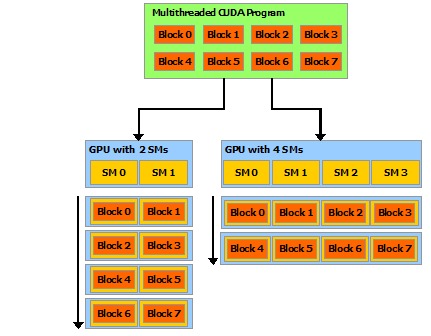
\includegraphics[width=\textwidth]{Documents/Report/Figures/Automatic scalability.png}
\caption{"Automatic scalability of thread blocks. Source: \cite[Figure 3]{nvidia:cudadoc}"}
\label{fig:automatic scalability}
\end{figure}

\begin{figure}[ht]
\includegraphics[width=\textwidth]{}
\caption{"Automatic scalability of thread blocks. Source: \cite[Figure 3]{nvidia:cudadoc}"}
\label{fig:automatic scalability}
\end{figure}
